\documentclass[conference]{IEEEtran}
\IEEEoverridecommandlockouts
% The preceding line is only needed to identify funding in the first footnote. If that is unneeded, please comment it out.
\usepackage{cite}
\usepackage{amsmath,amssymb,amsfonts}
\usepackage{algorithmic}
\usepackage{graphicx}
\usepackage{textcomp}
\usepackage{xcolor}
\usepackage{amsmath}
\usepackage{caption}
\usepackage{subcaption}
\usepackage{float}
\DeclareMathOperator*{\argmax}{argmax}

\usepackage{mathtools}
\newcommand\givenbase[1][]{\:#1\lvert\:}
\let\given\givenbase
\newcommand\sgiven{\givenbase[\delimsize]}
\DeclarePairedDelimiterX\Basics[1](){\let\given\sgiven #1}

\usepackage[
  separate-uncertainty = true,
  multi-part-units = repeat
]{siunitx}

\def\BibTeX{{\rm B\kern-.05em{\sc i\kern-.025em b}\kern-.08em
    T\kern-.1667em\lower.7ex\hbox{E}\kern-.125emX}}
\begin{document}

\title{H-1B Visa Approval Rate in the United States Analysis and Prediction using Machine Learning\\
}

\author{\IEEEauthorblockN{1\textsuperscript{st} Hao Yu}
\IEEEauthorblockA{\textit{Department of Electrical and Computer Engineering} \\
\textit{University of California, San Diego}\\
La Jolla, United States \\
hay024@ucsd.edu, A14050325}
\and
\IEEEauthorblockN{2\textsuperscript{nd} Kai Chuen Tan}
\IEEEauthorblockA{\textit{Department of Electrical and Computer Engineering} \\
\textit{University of California, San Diego}\\
La Jolla, United States \\
kctan@ucsd.edu, A59011493}
}

\maketitle

\begin{abstract}
H-1B visa is a temporary non-immigrant visa that allows highly-skilled foreign workers to work with U.S. employers legally, and H-1B visas play an important role in building and shaping the U.S. economy. The ever-increasing number of H-1B applicants every year and more imposed non-immigrant visa restrictions in the U.S. have significantly impacted highly-skilled foreign workers' American Dreams negatively to work long term in the U.S. As a result, the uncertainty of getting an H-1B for foreign workers and graduated international students in the U.S. rises, and it causes uncertainty in foreign workers' legal status in the U.S. Therefore, in this project, statistical methods are applied to perform pre-processing on the 2019 H-1B data-set from the U.S. Department of Labor website, and several machine learning and classifications techniques are implemented including Naive Bayes and K-Nearest Neighbor (KNN) Classifications to determine the correlation between the H-1B approval rate and features of several major categories. The project aims to help international students better plan which professions to select to maximize their probability of getting an H1-B visa sponsorship based on their field of study and interests.
\end{abstract}

\begin{IEEEkeywords}
H-1B Visa, H-1B Pre-processing Data, Naive Bayes Classification, K-Nearest Neighbor (KNN) Classification, Machine Learning
\end{IEEEkeywords}

\section{Background and Introduction}
\label{s1}
During the pre-COVID 19 eras, the United States (U.S.) non-immigrant visa restrictions and rules had made job-searching more challenging for international students, who studied and graduated from their United States institution \cite{b1}. The recent COVID-19 pandemic not only worsen the chances of a graduated international student from receiving a full-time job opportunity in the U.S. but also shattered the American dreams of highly-skilled foreign workers with an expiring H-1B visa due to the suspension of H-1B issuance by the Trump's administration in early July 2020 \cite{b2}. After the current U.S. President, Joe Biden won the 2020 U.S. Presidential Election and took over the office, the H-1B visa suspension was lifted in late March 2021, and employers could hire highly-skilled foreign workers again \cite{b3}. 

To make the college education spending worthwhile, most of the international graduates not only wanted to receive a world-class tertiary education and experience the diversity and culture in the U.S. but also eager to receive certain fields of job opportunities that might not be available in their home country and to gain valuable long-term work experience in the U.S. Nevertheless, a temporary non-immigrant, employment-based working visa, H-1B, is required for international graduates to work legally in the U.S. for a long term, and the annual H-1B visa limit is only 85,000 \cite{b4}. Out of 85,000 H-1B visas, 20,000 H-1B visas are reserved for applicants who are holding a master's degree or higher, and the remaining 65,000 H-1B visas are for any applicants including those who are holding an advanced degree; among 65,000 H-1B visas, 6,800 H-1B visas (i.e., H-1B1 Chile, and H-1B1 Singapore) are reserved for 1,400 applicants from Chile and 5,400 applicants from Singapore, respectively, and 10,500 H-1B visas (i.e., E-3 Australian) are reserved for applicants from Australia \cite{b5}. If the H-1B1 Chile, H-1B1 Singapore, and E-3 Australian are not used up in a particular year, they will be added back to the 65,000 H-1B visas cap. In order to apply for an H-1B visa, a foreign worker must be hired by an employer in the U.S., and the employer must be willing to sponsor the foreign worker an H-1B visa by submitting an H-1B visa petition to the U.S. Immigration Department.

The purpose of the "\emph{H-1B Visa Approval Rate in the United States Analysis and Prediction using Machine Learning}" project is to predict the probability of an international graduate or a foreign worker to get an H1-B visa application approved based on the degree-level completed, annual salary level, state of the worksite, job title, full-time position status, nationality, and company where the H1-B applicant works. Statistical methods will be applied to perform pre-analysis on the data, and several machine learning techniques will be implemented to determine the correlation between the result and features of each case. Eventually, the project would be able to help international students better plan which professions to select to maximize their probability of getting an H1-B visa sponsorship based on their field of study and interests.

\section{Data-Set Description}
\label{s2}

The year 2019 H-1B data-set was downloaded from the U.S. Department of Labor (DOL) official website \cite{b6}, and the data-set has 664,616 rows, which represents the total number of H-1B visa applicants, and 260 columns, which are known as categories including the case status, visa class, job title, etc. In this project, 8 out of 260 categories are selected from the data because the other categories are redundant like the decision date, prevailing wage tracking number, preparer last name, etc. Hence, the 8 categories that are focused on in this project are case status, visa class, Standard Occupational Classification (SOC) title, full-time position status, employer name, first worksite state, pay wage level, and statutory basis.

\section{Data Analysis and Visualization}
\label{s3}

The 9 main categories from the H-1B data-set as stated in the Data Description section are analyzed to gain some valuable insights from the data.

\textbf{H-1B Visa Case Status Analysis}: H-1B Case Status presents the outcome of an H-1B Visa application. The feature is extracted from the data-set, and there are 4 different possible classes or outcomes, which are Certified, Certified Withdrawn, Denied, and Withdrawn. In this project, only two main classes are taken into account, which are Certified and Denied, to do binary classification instead of multi-class classification. Hence, the two other classes (i.e., Certified-Withdrawn and Withdrawn) are converted into one of the two main classes as shown in \textbf{Fig.~\ref{fig_cs_1}}. Certified-Withdrawn and Withdrawn are considered as Denied in this project because they are not considered as a fully approved H-1B application.

\begin{figure}[htbp]
\centerline{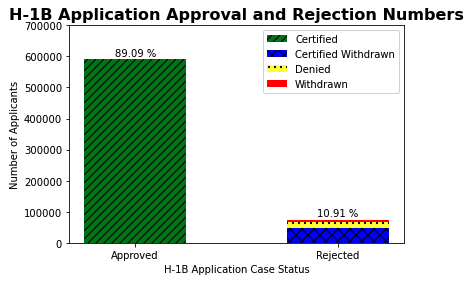
\includegraphics[scale = 0.5]{Case_Status.png}}
\caption{Numbers of Certified and Denied H-1B Applications}
\label{fig_cs_1}
\end{figure}

\textbf{Fig.~\ref{fig_cs_1}} illustrates that 89.09 \%-symbol of the 664,616 H-1B applications are certified, which are approximately 592,106, and only 10.91 \%-symbol H-1B applications are denied in year 2019. Based on the stacked bar chart in \textbf{Fig.~\ref{fig_cs_1}} above, H-1B applicants who filed and submitted their H-1B application, have a significantly high chance of getting their H-1B application certified.

\textbf{H-1B Visa Class Analysis}: H-1B Visa Class presents the type of H-1B visas that is submitted by an applicant for processing. As mentioned in \ref{s1}, H-1B Visas are divided into 4 different classes, which are the general H-1B, E-3 Australian, H-1B1 Chile, and H-1B1 Singapore. The percentages of certified and denied H-1B application for each visa class is shown below:

\begin{figure}[htbp]
\centerline{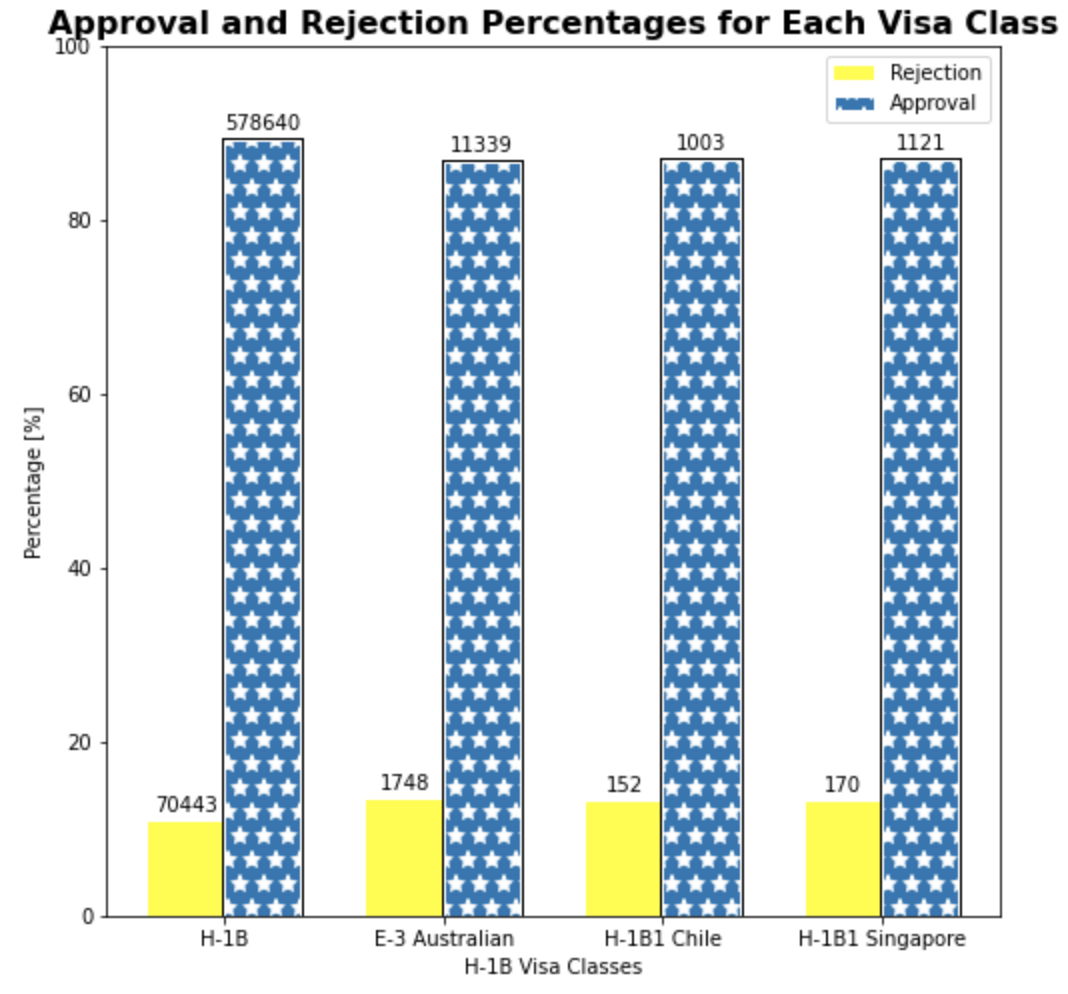
\includegraphics[scale = 0.30]{Visa_Class.png}}
\caption{Different H-1B Visa Classes' Certified and Denied H-1B Visas Percentages}
\label{fig_vc_1}
\end{figure}

\textbf{Fig.~\ref{fig_vc_1}} presents that all the different H-1B visa classes have approximately the same probability of getting the H-1B visa certified, which are around 86.0 \%-symbol to 89.0 \%-symbol, although the general H-1B visa class has the highest number of certified H-1B visa (i.e., 578,640), and the H-1B1 Chile has the lowest number of certified H-1B visa (i.e., 1,003). Hence, the data shows that there is no bias towards any visa class during the H-1B application process.

\textbf{Worksite State Analysis}: The Worksite State category from the H-1B visa application dataset presents the state in the U.S. where the H-1B applicant works. This category data information is crucial to analyze the number of H-1B applicants in each state in the U.S. because it provides insight about which states have more employers that are willing to sponsor H-1B visas for foreign workers as shown in the treemap below:

\begin{figure}[h]
\begin{subfigure}[h]{.3\textwidth}
\centering
% include first image
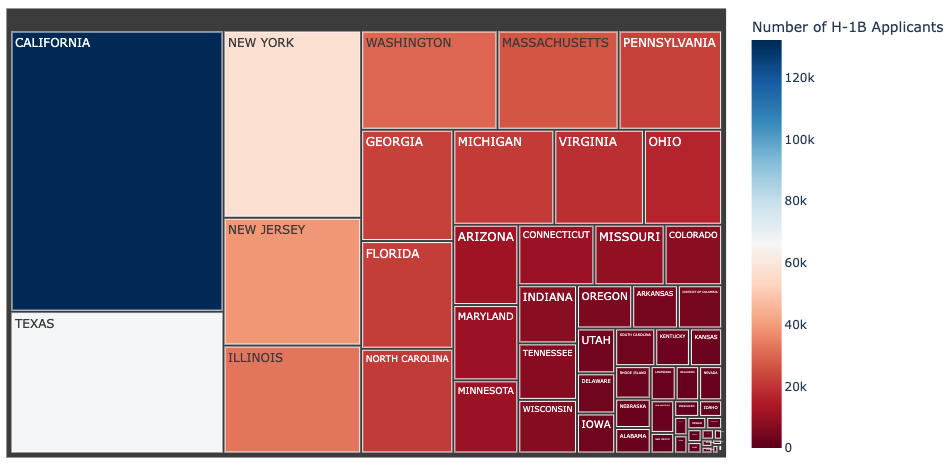
\includegraphics[scale=0.3]{State_NA.png}  
\end{subfigure}
\begin{subfigure}[h]{.3\textwidth}
\centering
% include second image
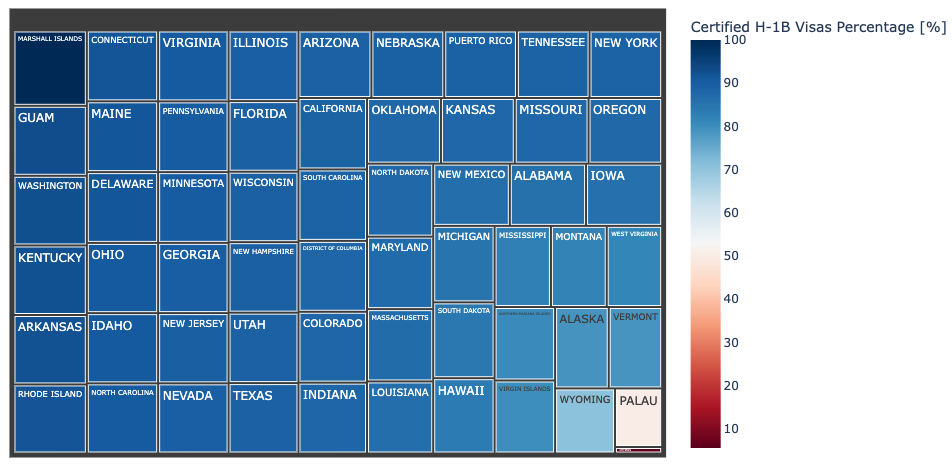
\includegraphics[scale=0.3]{State_Prob.png}  
\end{subfigure}
\caption{Number of H-1B Applicants in Different States (Top) and Percentage of Certified H-1B in Different States(Bottom)}
\label{fig_ws}
\end{figure}

According to \textbf{Fig.~\ref{fig_ws}} above, although California, Texas, and New York are the top three states in the U.S., where employers are willing to sponsor H-1B visas to highly-skilled foreign workers, most of the states have more than 80 \%-symbol of getting an H-1B visa certified except for Alaska, Wyoming, Vermont and Palau states as illustrated in \textbf{Fig.~\ref{fig_ws}}. The main reason that California state has the highest number of H-1B applicants is that majority of the Information Technology (I.T.) companies and the big tech companies like Facebook, Amazon, Apple, Netflix, Google, Tesla, and Microsoft Corporation are located there. Besides California, Texas and New York are second and third popular states, respectively, for highly-skilled foreign workers to work in the U.S.

\textbf{Employer Name Analysis}: Since knowing which employers hired and sponsored the most H-1B Visas for foreign workers are important to analyze, the employer name category information is extracted from the H-1B visa application data-set.

\begin{figure}[htbp]
\centerline{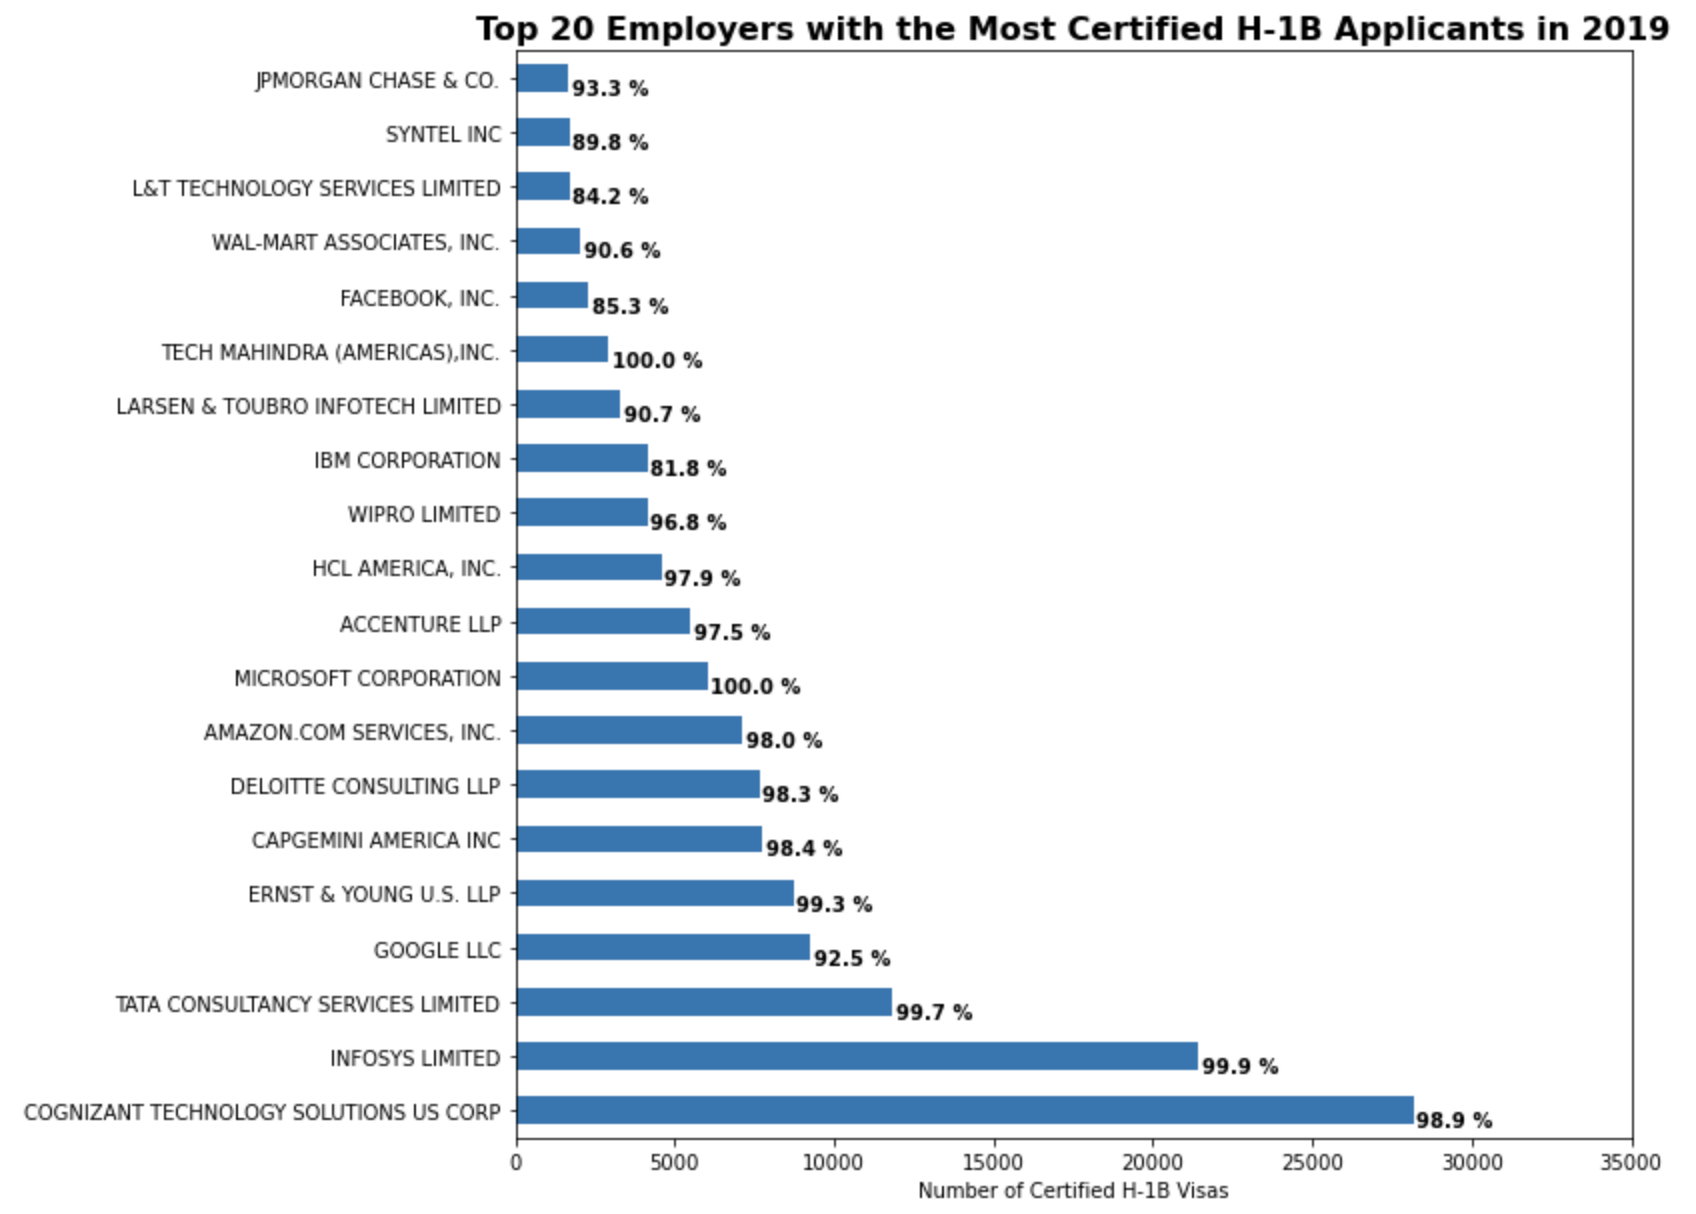
\includegraphics[scale = 0.28]{Employer_Name_20.png}}
\caption{Top 20 Companies that Sponsored the Most H-1B Visas}
\label{fig_en_1}
\end{figure}

\textbf{Fig.~\ref{fig_en_1}} shows that most of the employers who sponsored H-1B visas for foreign workers are I.T. companies like Google LLC, Amazon.com Services, Inc., Microsoft Corporation, Facebook, Inc., etc., and the top 3 employers are multinational consulting firms, which are Cognizant Technology Solutions US CORP, INFOSYS Limited, and TATA Consultancy Services Limited. Besides that, the H-1B visa application approval rate for the top 20 employers have more than 81.0 \%-symbol probability of getting an H-1B visa application certified; Microsoft Corporation and Tech Mahindra (Americas), Inc. have all of their H-1B visa applications certified in the year 2019.

\textbf{Job Position Type Analysis}: Job position type presents the information about whether the foreign worker will be working as a full-time or a part-time employee for the employer who sponsored the H-1B visa. The data provides insight about whether U.S. employers are preferred to sponsor H-1B visas for full-time or part-time employees.

\begin{figure}[htbp]
\centerline{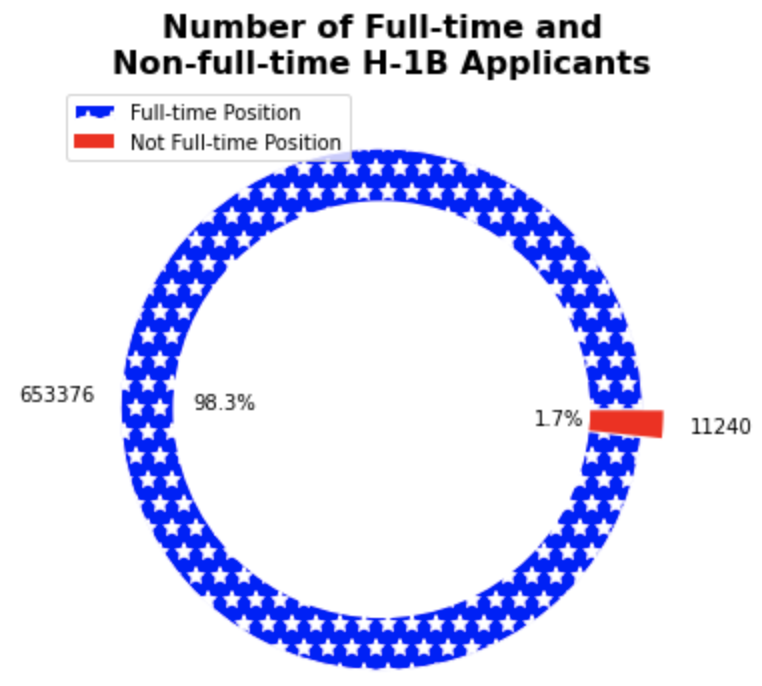
\includegraphics[scale = 0.5]{FT_NA.png}}
\caption{Number of Full-time and Part-time H-1B Applicants}
\label{fig_ft_nft_1}
\end{figure}

\textbf{Fig.~\ref{fig_ft_nft_1}} above illustrates 98.3 \%-symbol (i.e., 653,376 applicants) of the H-1B applications are working as a full-time employee, and only 1.7 \%-symbol (i.e., 11,240 applicants) of the H-1B applications are for the part-time positions. Hence, more employers preferred to sponsor H-1B visas for full-time employees rather than part-time employees.

\begin{figure}[h]
     \begin{subfigure}[h]{0.2\textwidth}
         \centering
         \hbox{\hspace{0em}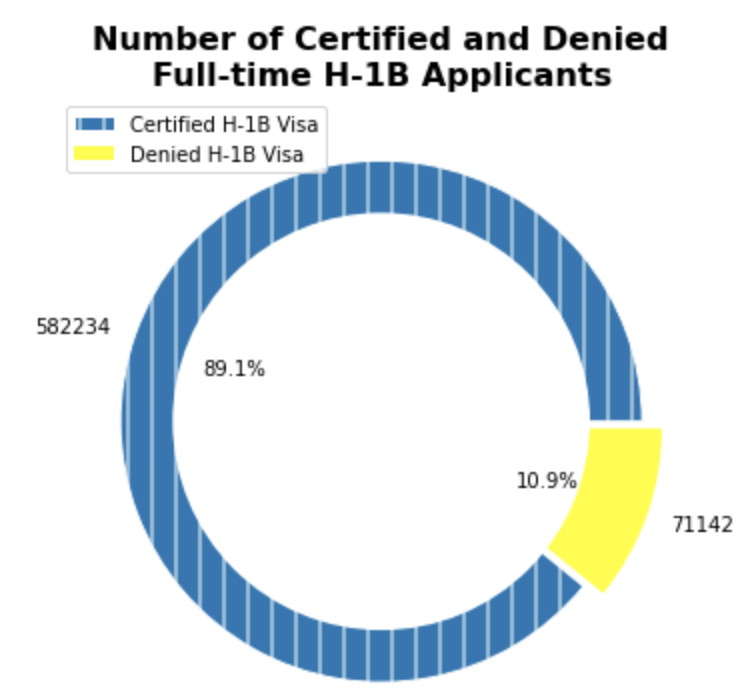
\includegraphics[scale = 0.3]{FT_Cert_Denied.png}}
     \end{subfigure}
     \hfill
     \begin{subfigure}[h]{0.2\textwidth}
         \centering
         \hbox{\hspace{-8em}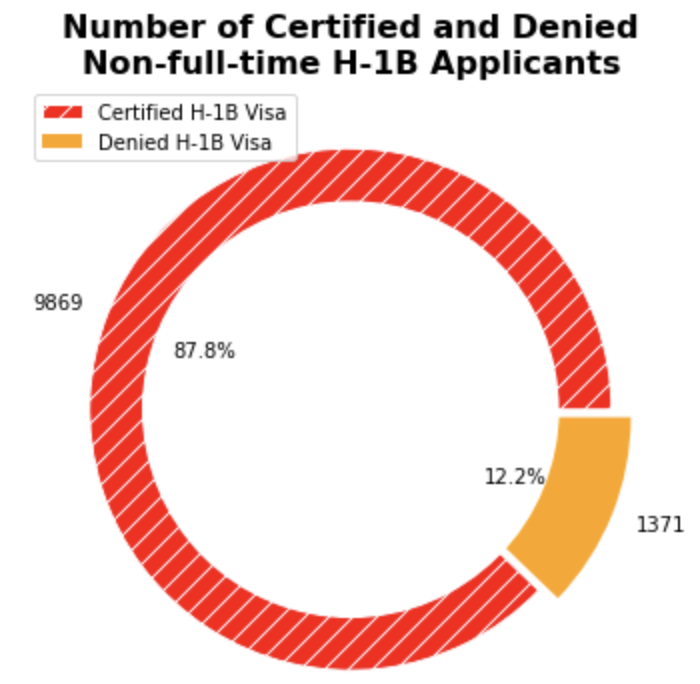
\includegraphics[scale=0.3]{NFT_Cert_Denied.png}}
     \end{subfigure}
        \caption{Difference Between Full-time and Part-time H-1B Applicants}
        \label{Fig_ft_nft_2}
\end{figure}

Although there are more H-1B visa applications for full-time positions than part-time positions, the percentage of certified H-1B visa application for full-time jobs are just 1.3 \%-symbol higher than the percentage of certified H-1B visa application for part-time positions, which are 87.8 \%-symbol (i.e., 9,869 out of 11,240 part-time H-1B applicants) as shown in \textbf{Fig.~\ref{Fig_ft_nft_2}}. Therefore, the job position type does not affect much the probability of getting an H-1B visas application certified.

\textbf{Prevailing Wage Level Analysis}: Prevailing Wage Level is defined as the range of foreign workers' wages paid by the employer, and it is divided into four levels, which are Level I, Level II, Level III, and Level IV. H-1B Wage Level I (entry) annual salary ranges from USD 38k to USD 51k; H-1B Wage Level II (qualified) annual salary ranges from USD 51k to USD 65k; H-1B Wage Level III (experienced) annual salary ranges from USD 65k to USD 75k; H-1B Wage Level IV (Fully Competent) annual salary ranges from USD 78k to USD 90k \cite{b7}. The information from this category provides an insight about which Prevailing Wage Level has the most H-1B visa applications, and how it affects the probability of getting the H-1B application certified.

\begin{figure}[htbp]
\centerline{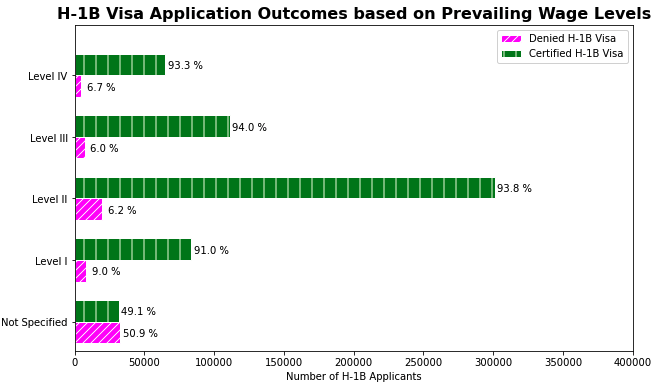
\includegraphics[scale = 0.3]{PWL.png}}
\caption{Relationship between H-1B Case Status and Prevailing Wages Level}
\label{fig_pwl}
\end{figure}

\textbf{Fig.~\ref{fig_pwl}} shows that Prevailing Wage Level II has the largest number of certified H-1B applications, which is 301,168, and H-1B applications that do not specify prevailing wage level has the lowest number of certified H-1B visas (i.e., 31,417). As long as the prevailing wage level is specified in the H-1B application, all the prevailing wage levels have more than 90.0 \%-symbol of getting an H-1B visa application certified. If the prevailing wage level is not specified in the H-1B visa application, it is more likely to get an H-1B application denied, which is 50.9 \%-symbol. Hence, the \textbf{Fig.~\ref{fig_pwl}} presents that employers are more willing to sponsor H-1B visas for foreign workers who have more work experience, but the work experience or prevailing wage level does not affect the chances of getting an H-1B visa application approved.

\textbf{Statutory Basis Analysis}: Statutory basis presents information about whether the H-1B visa application has either an advanced degree, USD 60k annual salary or higher, both, or none. In this project, we only focused on whether the applicant has an advanced degree or not; hence, "USD 60k Annual Salary" and "None" are classified as an applicant without an advanced degree, and "Advanced Degree" and "Both" are classified as an applicant with an advanced degree

\begin{figure}[htbp]
\centerline{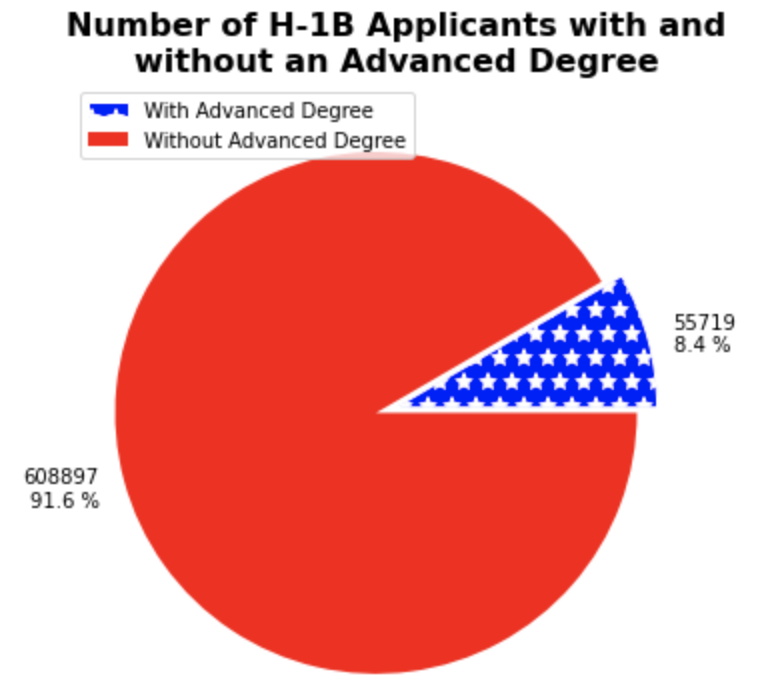
\includegraphics[scale = 0.35]{ADV_Deg.png}}
\caption{Number of H-1B Applicants with and without Advanced Degree}
\label{fig_adv_nadv_1}
\end{figure}

\textbf{Fig.~\ref{fig_adv_nadv_1}} illustrates that the number of H-1B visa applications without an advanced degree is 10.9 times more than the number of H-1B visa applications with an advanced degree. The data also show most of the occupations do not really require an advanced degree to qualify for a job position. 

\begin{figure}[h]
     \begin{subfigure}[h]{0.2\textwidth}
         \centering
         \hbox{\hspace{0em}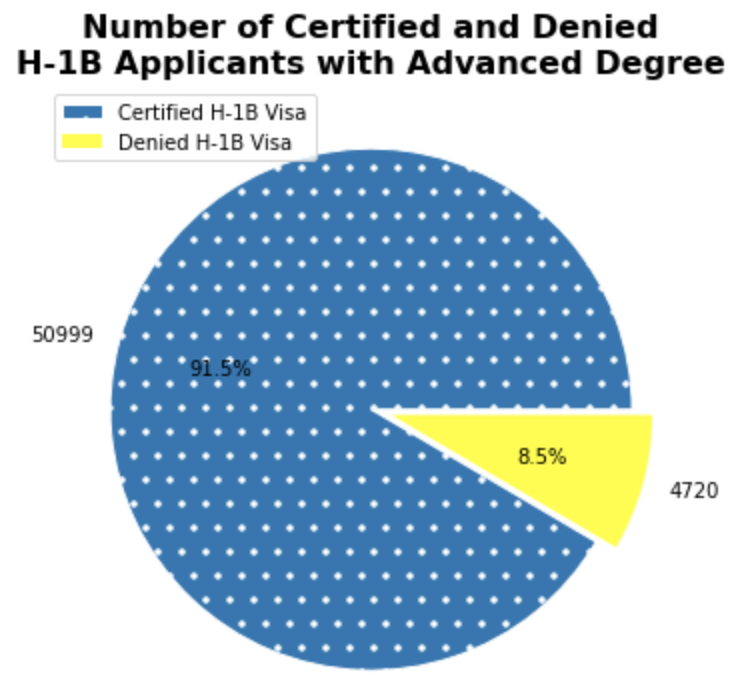
\includegraphics[scale = 0.3]{Cert_Den_Adv.png}}
     \end{subfigure}
     \hfill
     \begin{subfigure}[h]{0.2\textwidth}
         \centering
         \hbox{\hspace{-8em}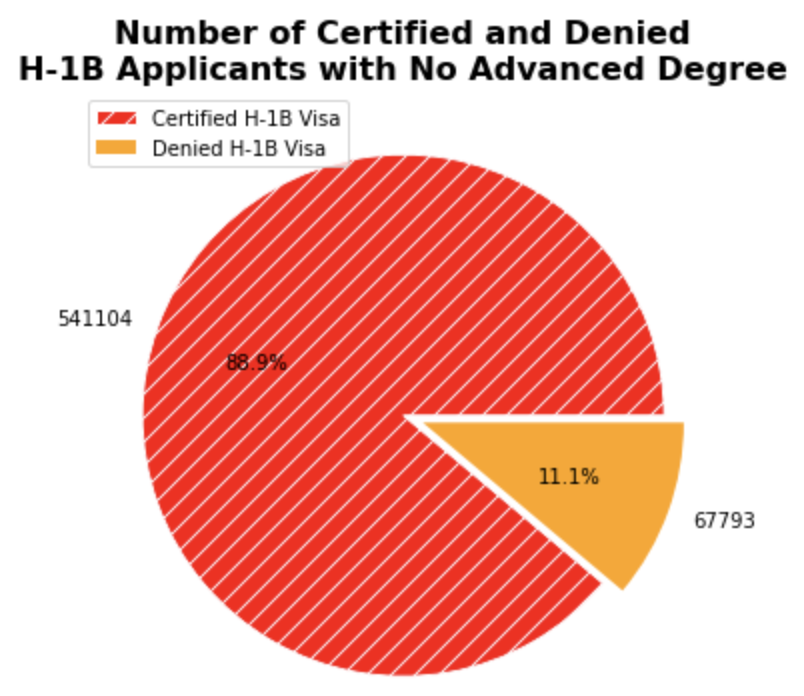
\includegraphics[scale=0.3]{Cert_Den_nAdv.png}}
     \end{subfigure}
        \caption{Difference Between H-1B Applicants with and without Advanced Degree}
        \label{fig_adv_nadv_2}
\end{figure}

According to the \textbf{Fig.~\ref{fig_adv_nadv_2}}, H-1B applications with an advanced degree just have 2.6 \%-symbol higher chances of getting an H-1B visa application certified than H-1B applications without an advanced degree. Nevertheless, both H-1B visa applications with and without an advanced degree have a very probability of getting the H-1B visa application certified, which are 91.5 \%-symbol and 88.9 \%-symbol, respectively. Therefore, an H-1B visa application with an advanced degree does not significantly improve the chances of getting an H-1B visa application certified.

\textbf{Standard Occupational Classification (SOC) Title Analysis}: Standard Occupational Classification (SOC) Title classifies foreign workers' job titles into a more general occupational category, for example, mechanical design engineer and mechanical systems control engineer are classified as mechanical engineers. SOC title from the data-set provides insight about which occupational categories have the most H-1B visa applications. The top 20 SOC titles with the most certified H-1B visa are filtered and plotted to analyze as shown in the figure below.

\begin{figure}[htbp]
\centerline{\hbox{\hspace{1em}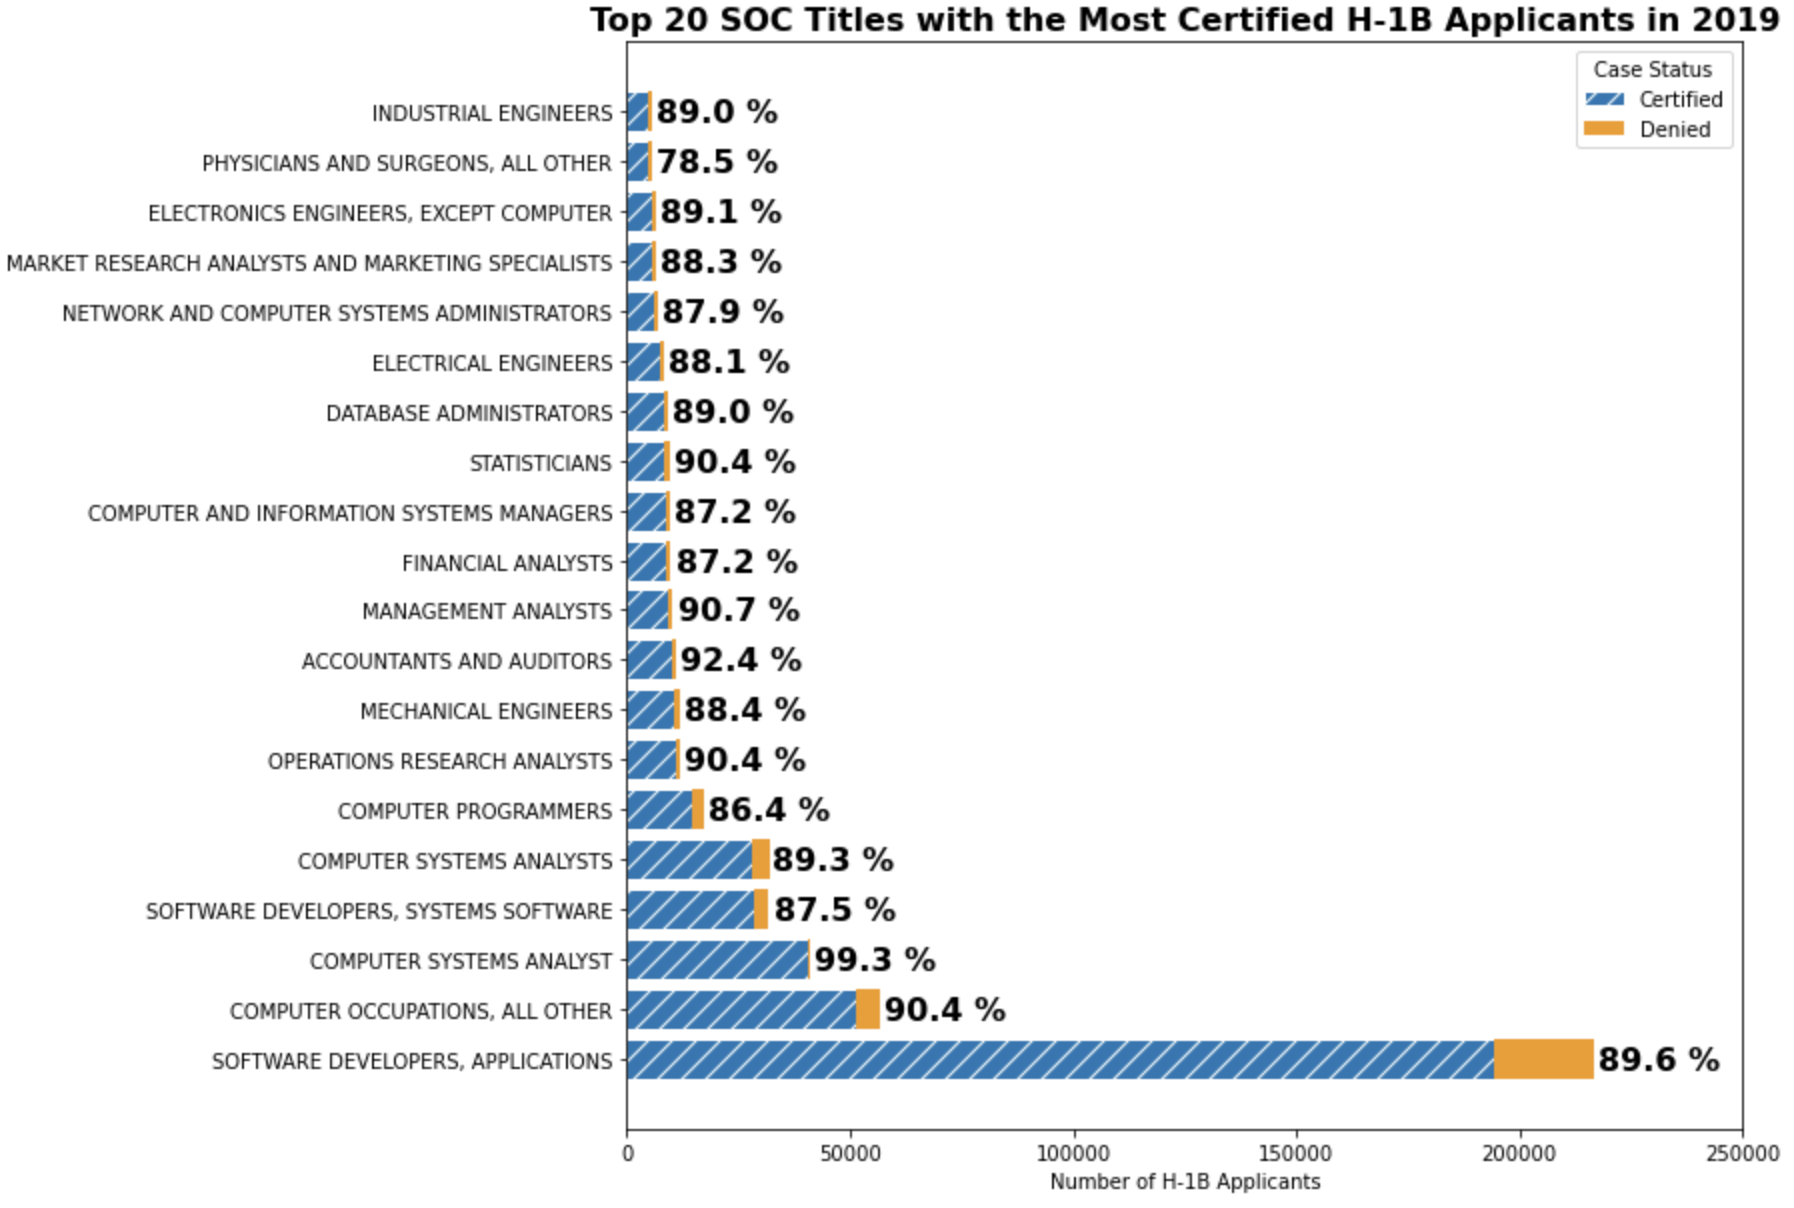
\includegraphics[scale = 0.3]{SOC_Title.png}}}
\caption{Top 20 SOC Titles in H-1B Applications}
\label{fig_soc}
\end{figure}

\textbf{Fig.~\ref{fig_soc}} illustrates that the top 3 occupational categories that have the most H-1B visa applications are "Software Developers, Applications", "Computer Occupations, All Other", and "Computer System Analysis", and the top 20 occupational categories are mostly in the field of I.T. "Electrical Engineer" is in the top 15 occupational categories with 7,316 certified H-1B visa applications, but it is 96.2 \%-symbol less than the top one occupational category (i.e., Software Developers, Applications) number of certified H-1B visa applications (i.e., 194,060 certified H-1B visa applications). Hence, the data presents that there are significantly more job opportunities in the I.T. field for highly-skilled foreign workers. However, most of the top 20 SOC titles have more than 85.0 \%-symbol chance of getting an H-1B visa application certified, except for the "Physicians and Surgeons, All Other" occupational category.

\section{Logistical Prediction}

After we have finished pre-processing the data, we perform statistical analysis on the data to predict the probability that an international student receives an H-1B visa. Since there are only two outcomes for the event of H-1B visa application (approved or denied), we decided to build logistical models to fit the data we have and utilize those logistical models to make predictions afterwards. In order to check the accuracy of our models, we split the data randomly into training data and testing data by a four over one distribution, and we call them \(X_{train}\) and \(X_{test}\), accordingly. We also extract the results of corresponding cases in both \(X_{train}\) and \(X_{test}\), can we call them \(y_{train}\) and \(y_{test}\).
\subsection{Models}

Two models were applied in this project to fit the pre-processed data and make predictions about future possible cases, which are Naïve Bayes classifier model \cite{b8} and K-Nearest Neighbour classifier model \cite{b9}. 

\hfill\\

\subsubsection{Naïve Bayes Classifier}

The first model implemented is a Naïve Bayes classifier model. Based on the Bayes' theorem \cite{b10}, 
\[P(A \given B) = \frac{P(B \given A) P(A)}{P(B)} \]
a Naïve Bayes classifier is capable of generating strong independence relationships among features. In this particular project, we applied the Naïve Bayes classifier to generate logistical assumptions from the set \[C = \{\emph{Denied}, \emph{Certified} \}\]

We take another step and mark the word \emph{Denied} as 0, \emph{Certified} as 1, which leads the set of the assumption result to be \(C = \{0, 1 \}\). 
In order to fit data of words into the Naïve Bayes classifier, a binary bag of word (BoW) \cite{b11}  matrix needs to be built. We first collect all the unique words in the attributes of the selected features, and store them in a set \(D\), where \(d\) denotes the size of the set. We then treat features in each case as words in an independent sentence, and we represent features in each case by a binary vector \(x_n\), where \[x_n \in \{0, 1\}^d\]
here, \(x_n[d] = 1 \) means the n-th element in \(X_{train}\) contains the d-th unique word in the word set \(D\), and \(x_n[d] = 0 \) means the n-th element in \(X_{train}\) does not contain the d-th unique word in the word set \(D\). 

After we have presented every case in \(X_{train}\) as a d-dimensional binary vector, we then build the Naïve Bayes classifier and train it. To achieve this, we first build a \(2 \; by \; d\) matrix filled with zero and called it \(S\). After that, we loop through all cases in \(X_{train}\) and create a d-dimensional binary vector, \(x\), for each case. For each \(x\), we get the corresponding \(y_{train}\) data, \(Y\) for that particular case and updated the matrix \(S\) we just created

\[S[Y, i] = S[Y, i] + x[i], \; for \; i \in \{0, 1, 2, ..., d - 1\} \]

After we have finished updating the matrix \(S\) using \(X_{train}\) and \(y_{train}\), we applie the maximum likelihood estimation (MLE) method to predict result for cases in \(X_{test}\) to get the analysis the accuracy of the model we built [CITE SOMETHING]. For each case in \(X_{test}\), we converte it to a d-dimensional vector as we did for cases in \(X_{train}\), and we call it \(x\). For each x, we calculate the prediction result \(y_{pred}\) by 

\[y_{pred} = \argmax_{C=\{0, 1\}} \prod_{i = 1}^{d} p(x[i] \given Y = C) \; p(Y = C)\]
\[= \argmax_{C=\{0, 1\}} \prod_{i = 1}^{d} S[Y, i] \; p(Y = C)\]

However, some elements in \(x\) had a numerical value of 0, which means that particular case didn't contain a unique word in the set \(D\), and it would lead \(y_{pred}\) to zero. To solve this problem, we calculate \(log\) of the expression of \(y_{pred}\) instead of \(y_{pred}\) itself

\[y_{pred} = \argmax_{C=\{0, 1\}} \; \log\prod_{i = 1}^{d} S[Y, i] \; p(Y = C)\]
\[y_{pred} = \argmax_{C=\{0, 1\}} (\sum_{i = 1}^{d} \log S[Y, i] \; + \log p(Y = C) )\]

The value \(y_{pred}\) illustrates the result of prediction for a particular case, \(x\), in \(X_{test}\). By performing the same procedure to every case in \(X_{test}\), we predict the results for all cases in \(X_{test}\) and collect the prediction results. 

\hfill\\

\subsubsection{K-Nearest Neighbours Classifier}

The second model implemented is a K-Nearest Neighbour (KNN) classifier model. The KNN algorithm is a data classification method that predicts which group a data point will become a member of based on the distance between that data point and k nearest data points in the available groups. Different from Naïve Bayes classifier, KNN is a lazy classification algorithm, which means training doesn't take place while we implement KNN algorithm. However, the initial infrastructure processes for data using Naïve Bayes and KNN algorithms are similar. For both algorithms, we create the BoW, split the raw data into training and testing sets similar to what we did for when we implemented the Naïve Bayes classifier. After getting \(X_{train}\), \(y_{train}\), \({X}_test\), \({y}_test\), for each case in \(X_{set}\), we get the binary vector, \(x_d\), and we calculate the euclidean distances between \(x_d\) and all binary vectors in \(X_{train}\). We sort the calculated distances, find k smallest distances and their corresponding cases. We record the logistical results of those cases, and vote the most common result. For example, if we choose k to be 3. Then for a random \(x_d\) in \(X_{set}\), we will find the 3 cases that have the shortest distance from \(x_d\). Assuming the three generated results are \({"Denied", "Accepted", "Accepted"}\). then the prediction for \(x_d\) will be "Accepted". We perform the above action for every case in the test set, and get the \(y_{pred}\), and we evaluate the accuracy of prediction by comparing \(y_{pred}\) and \(y_{test}\). 


\subsection{Prediction}

After performing the Naive Bayes analysis on the pre-processed data, the accuracy for predicting was calculated to be 87.90 \%-symbol. The confusion matrix and table of conditional probability for prediction are shown below. 

\begin{figure}[htbp]
\centerline{\hbox{\hspace{1em}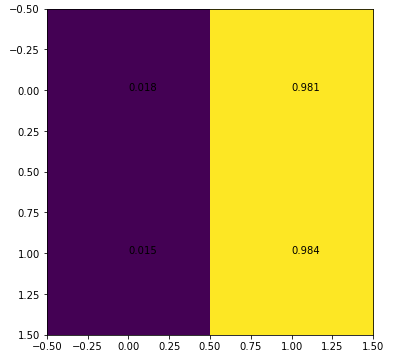
\includegraphics[scale = 0.5]{confus_naive.png}}}
\caption{Confusion Matrix for Naive Bayes Classification}
\label{fig_con_n}
\end{figure}

\textbf{Fig.~\ref{fig_con_n}} illustrates the confusion matrix for the result of prediction using the Naive Bayes classifier. The rows represent the ground truth result, where the first row indicates "Denied", and the second row indicates "Accepted". The columns represent the prediction result, where the first column shows "Denied", and the second column shows "Accepted". The number in the figure means the probability of truth/false - positive/negative. For example, the number in second row second column, 0.984, tells the probability that 98.4 \%-symbol cases that are labeled "Accepted" also get predicted to be "Accepted" in this model. 

\hfill\\

\begin{figure}[htbp]
\centerline{\hbox{\hspace{1em}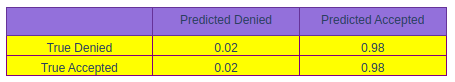
\includegraphics[scale = 0.5]{naive_bayes.png}}}
\caption{Conditional Probability for Predicting Results}
\label{fig_tab_n}
\end{figure}

\textbf{Fig.~\ref{fig_tab_n}} represents the conditional probability explicitly for the Naive Bayes model. 

Accuracy of applying the KNN algorithm was figured out to be 88.13 \%-symbol when k is defined to be 5. The confusion matrix and table of conditional probability for prediction are shown below. 

\begin{figure}[htbp]
\centerline{\hbox{\hspace{1em}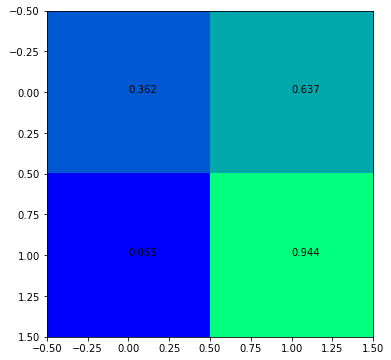
\includegraphics[scale = 0.5]{confus_knn.png}}}
\caption{Confusion Matrix for K-Nearest Neighbours Classification}
\label{fig_con_k}
\end{figure}

\textbf{Fig.~\ref{fig_con_k}} illustrates the confusion matrix for the result of prediction using the KNN classifier. The rows represent the ground truth result, where the first row indicates "Denied", and the second row indicates "Accepted". The columns represent the prediction result, where the first column shows "Denied", and the second column shows "Accepted". The number in the figure means the probability of truth/false - positive/negative. 

\hfill\\

\begin{figure}[htbp]
\centerline{\hbox{\hspace{1em}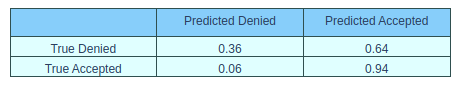
\includegraphics[scale = 0.5]{knn.png}}}
\caption{Conditional Probability for Predicting Results}
\label{fig_tab_k}
\end{figure}

\textbf{Fig.~\ref{fig_tab_k}} represents the conditional probability explicitly for the KNN model. 

\hfill\\

\begin{figure}[htbp]
\centerline{\hbox{\hspace{1em}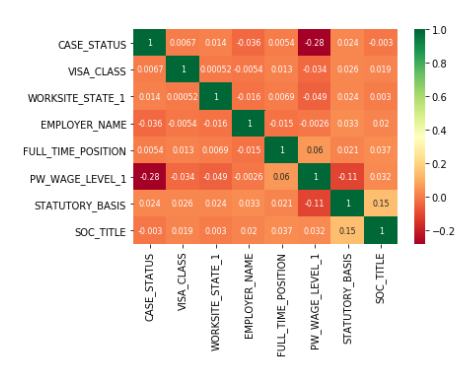
\includegraphics[scale = 0.5]{corr.png}}}
\caption{Correlation Between the Selected Features and Ground Truth Results}
\label{corr}
\end{figure}

\textbf{Fig.~\ref{corr}} illustrates the correlation between the selected features and the application result. In this figure, the greenish colors indicate high correlation between subjects, and reddish colors indicate low correlation between subjects. 


\subsection{Discussion of Prediction Results}
In order to find the optimal number for the number of neighbours, k, multiple k was experimented, including 1, 3, 5, 7, and 9. Among the results produced, \(k = 5\) provided the optimal accuracy. However, values of accuracy using other k are not ideal. For example, accuracy of prediction when k was defined to be 3 was found to be 41.02 \%-symbol, which was assumed to be unacceptable. 

Even though the accuracy found by applying the optimal k for the KNN algorithm, 88.13 \%-symbol, leaded to a better result than the result generated by the Naive Bayes classifier, 87.90 \%-symbol, it is not larger than 1 \%-symbol, thus the advantage is considered to be trivial. By observing the conditional probability, we found that both models have a strong bias towards generating results labeled as "Approved". One possible explanation is this data set contains significantly more cases labeled as "Approved" than "Denied". By analyzing the raw data, only 10.85 \%-symbol cases were labeled as "Denied", which indicated that number of cases labeled as "Approved" is 9 times the number of cases labeled as "Denied". Another possible explanation is there are no strong correlations between the features we selected and the results. From {Fig.~\ref{corr}}, we can tell that the correlation between subjects we selected and the final results are small. Two assumptions were made to explain the low correlations. Perhaps we didn't select the most outstanding features, perhaps results of applications of H-1B Visa was randomly distributed. 


\section{Conclusion}

H-1B Visa is a significant component of the U.S. economy, and it has strong effect on international students who have career plans of working in the U.S. after graduation. This project analyzed on the 2019 H-1B cases and it focused on predicting the probability of getting certified for entering the H-1B lottery based on some features that are assumed to play an important role in the application. As a conclusion, even though this project failed find a dominant feature that will effect greatly effect the result of applications, two models used for predicting the results achieved an accuracy close to 90 percent. In addition, visualization on the raw data shows that the probability of getting certified was 89 percent. Combining the two results, this project would encourage any international students who desires to start a career in the U.S. to apply for the H-1B Visa due to its high certified probability and low bias towards a specific field.  

% \section{References}

\begin{thebibliography}{00}
\bibitem{b1} M. Krislov, “Why international students are good for colleges, Universities and America,” Forbes, 22-Mar-2019. [Online]. Available: https://www.forbes.com/sites/marvinkrislov/2019/03/22/why-international-students-are-good-for-colleges-universities-and-america/?sh=612fb786f496. [Accessed: 23-Nov-2021]. 
\bibitem{b2} V. Gewin, “The visa woes that Shattered Scientists' american dreams,” Nature News, 28-Sep-2020. [Online]. Available: https://www.nature.com/articles/d41586-020-02746-y. [Accessed: 23-Nov-2021]. 
\bibitem{b3} J. Fabian and G. Douglas, “Biden to Let Trump’s H-1B Visa Ban Expire in Win for Tech,” Bloomberg.com, 30-Mar-2021. [Online]. Available: https://www.bloomberg.com/news/articles/2021-03-30/biden-to-let-trump-s-h1-b-visa-ban-expire-in-win-for-tech-firms. [Accessed: 23-Nov-2021].
\bibitem{b4} S. Anderson, “2021 might be a decisive year for H-1B Visas,” Forbes, 02-Jun-2021. [Online]. Available: https://www.forbes.com/sites/stuartanderson/2021/06/02/2021-might-be-a-decisive-year-for-h-1b-visas/?sh=1d708d6118df. [Accessed: 23-Nov-2021]. 
\bibitem{b5} “H-1B, H-1B1 and E-3 Specialty (Professional) Workers,” United States Department of Labor. [Online]. Available: https://www.dol.gov/agencies/eta/foreign-labor/performance. [Accessed: 25-Nov-2021]. 
\bibitem{b6} “Performance data,” United States Department of Labor. [Online]. Available: https://www.dol.gov/agencies/eta/foreign-labor/performance. [Accessed: 25-Nov-2021]. 
\bibitem{b7} Yekrangi &amp; Associates. (2021, April 9). What are the wage levels for H1-B visa workers? Yekrangi; Associates. Retrieved December 4, 2021, from https://www.yeklaw.com/blog/2021/april/what-are-the-wage-levels-for-h1-b-visa-workers-/. 
\bibitem{b8} McCallum, Andrew, and Kamal Nigam. "A comparison of event models for naive bayes text classification." AAAI-98 workshop on learning for text categorization. Vol. 752. No. 1. 1998.
\bibitem{b9}Guo, Gongde, et al. "KNN model-based approach in classification." OTM Confederated International Conferences" On the Move to Meaningful Internet Systems". Springer, Berlin, Heidelberg, 2003.
\bibitem{b10}Swinburne, Richard. "Bayes' Theorem." Revue Philosophique de la France Et de l 194.2 (2004).
\bibitem{b11}Sethy, Abhinav, and Bhuvana Ramabhadran. "Bag-of-word normalized n-gram models." Ninth Annual Conference of the International Speech Communication Association. 2008.
\end{thebibliography}
% \vspace{12pt}
% \color{red}
% IEEE conference templates contain guidance text for composing and formatting conference papers. Please ensure that all template text is removed from your conference paper prior to submission to the conference. Failure to remove the template text from your paper may result in your paper not being published.

\end{document}
